\documentclass{beamer}

\usepackage[utf8]{inputenc}
\usepackage[T1]{fontenc}
\usepackage[french]{babel}
\usepackage[ddmmyyyy]{datetime}

\usetheme{Warsaw}
\useinnertheme{rectangles}
\setbeamerfont{headline}{size=\large}
\setbeamerfont{frametitle}{size=\normalsize}

%Plan/Sommaire automatique avant chaque section
\AtBeginSection[]{
  \begin{frame}
  \frametitle{Plan}
  \tableofcontents[currentsection]
  \end{frame}
}

\author{Sonny Klotz - Jean-Didier Pailleux - Malek Zemni}
\institute{UVSQ}
\date{\today}
\usepackage{../tex/myInfolines}
\title{Présentation Cahier des Charges}

\begin{document}

	\begin{frame}
		\titlepage
	\end{frame}
	
	\begin{frame}
		\frametitle{Plan général}
		\tableofcontents
	\end{frame}
	
	\section{Introduction}
	\begin{frame}
		Malek
	\end{frame}
	
	\section{Motivations}
	\begin{frame}
		Malek
	\end{frame}	
	
	\section{Contraintes}
	\begin{frame}
		Malek
	\end{frame}
	
	\section{Exigences fonctionnelles}
	\begin{frame}
		Sonny
	\end{frame}
	
	\section{Exigences fonctionnelles}
	\begin{frame}
		\begin{center}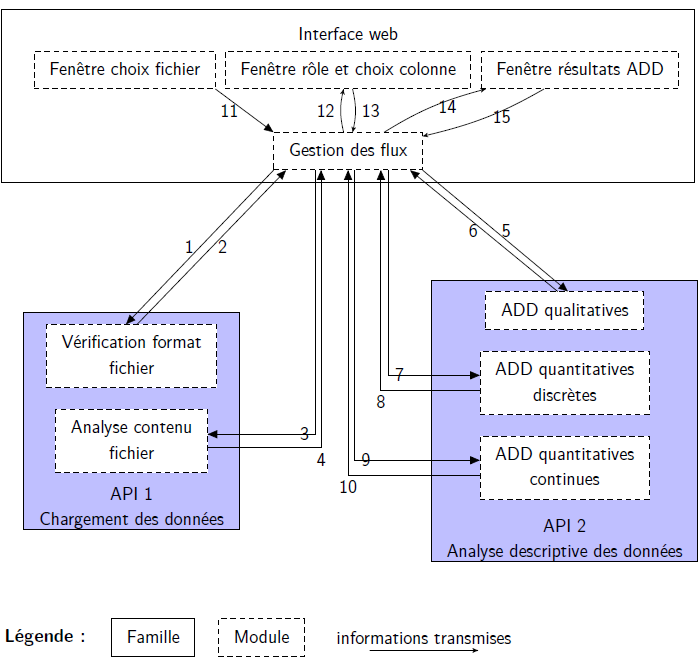
\includegraphics[scale=0.43]{org.png}\end{center}
	\end{frame}
	
	\section{Exigences non fonctionnelles}
	\begin{frame}
		Jean-Édouard
	\end{frame}
	
	\section{Autres aspects}
	\begin{frame}
		Jean-Claude
	\end{frame}
	
	\section{Conclusion}
	\begin{frame}
		Jean-Claude Van Damme
	\end{frame}
	
\end{document}
